
\chapter{Instalación de la máquina virtual}

Para realizar la práctica creamos la máquina virtual NFS-anabuenrua, que tendrá, al igual que las otras, 1GB de RAM y 10GB de disco duro dinámico. Además, se ha añadido antes de lanzar la máquina virtual el adaptador de red solo-anfitrión. Introducimos los datos como puede verse en \eqref{instal_1}.

\begin{figure}[h!]
\begin{center}
\caption{Introducimos los datos de la máquina virtual durante la instalación.}
\label{instal_1}
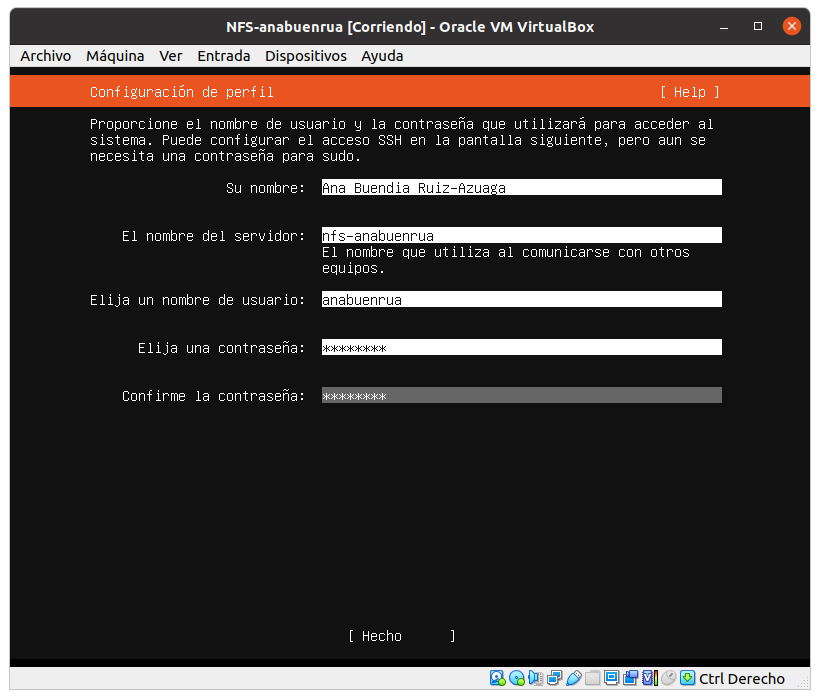
\includegraphics[scale=0.5]{instal_1}
\end{center}
\end{figure}

Ahora asignamos una IP estática a nfs-anabuenrua, se ha escogido 192.168.56.105 editando \verb|/etc/netplan/00-installer-config.yaml|, por tanto, el fichero quedaría como en \eqref{instal_2}.

\begin{figure}[h!]
\begin{center}
\caption{Fichero /etc/netplan/00-installer-config.yaml}
\label{instal_2}
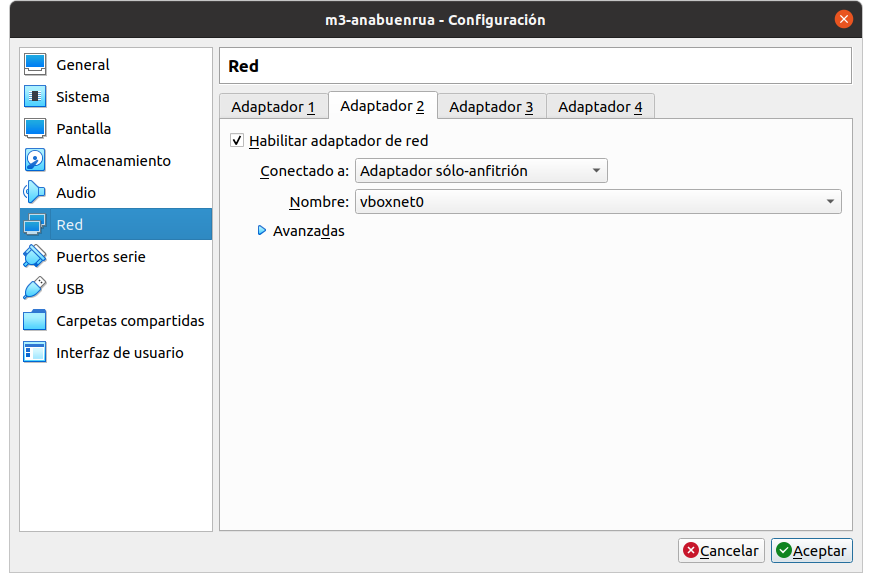
\includegraphics[scale=0.5]{instal_2}
\end{center}
\end{figure}

Hacemos los cambios efectivos ejecutando \verb|sudo netplan apply| como en las prácticas anteriores y comprobamos que hay conexión en \eqref{instal_3}.

\begin{figure}[h!]
\begin{center}
\caption{Comprobación de la conexión de la máquina con otras máquinas.}
\label{instal_3}
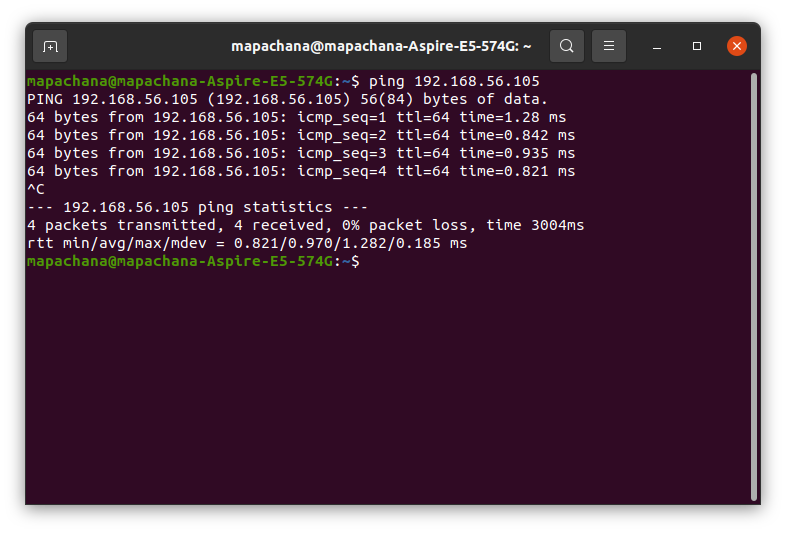
\includegraphics[scale=0.5]{instal_3}
\end{center}
\end{figure}

\chapter{Configurar servidor de disco NFS}

Comenzamos la práctica trabajando en nfs-anabuenrua. Primero instalamos las herramientas básicas que vamos a necesitar ejecutando el comando de \eqref{config_1}.

\begin{figure}[h!]
\begin{center}
\caption{Instalación de herramientas en nfs-anabuenrua}
\label{config_1}
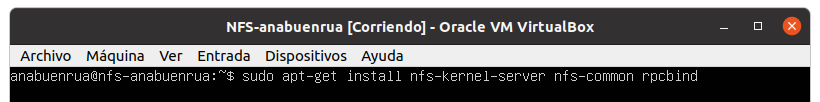
\includegraphics[scale=0.5]{config_1}
\end{center}
\end{figure}

Ahora creamos la carpeta \verb|/datos/compartido| donde vamos a tener los ficheros que se van a compartir entre las máquinas virtuales, cambiamos su propietario y grupo y asignamos permisos, como mostramos en \eqref{config_2}.

\begin{figure}[h!]
\begin{center}
\caption{Creación de carpeta /datos/compartido, cambio de propietarios y asignación de permisos.}
\label{config_2}
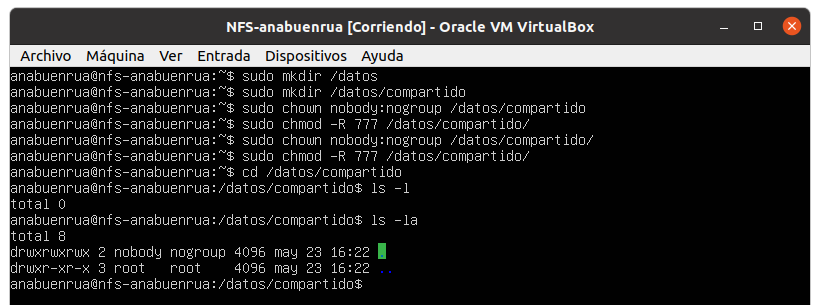
\includegraphics[scale=0.5]{config_3}
\end{center}
\end{figure}

A continuación editamos \verb|/etc/exports| para dar permisos de acceos a m1 y m2, como se ve en \eqref{config_4}.

\begin{figure}[h!]
\begin{center}
\caption{Fichero /etc/exports.}
\label{config_4}
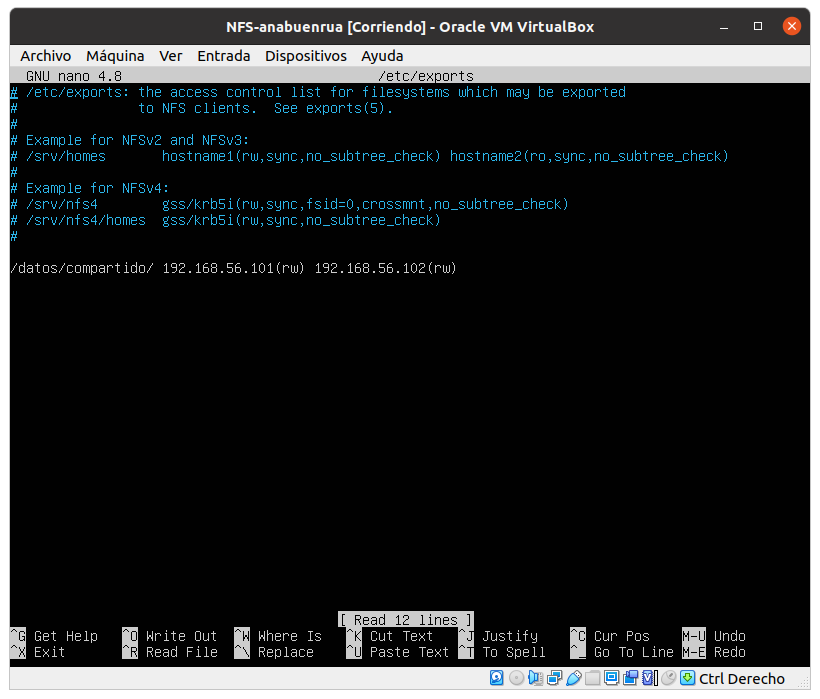
\includegraphics[scale=0.5]{config_4}
\end{center}
\end{figure}

Finalmente relanzamos el servicio y comprobamos su estado. Esto puede consultarse en \eqref{config_5}.

\begin{figure}[h!]
\begin{center}
\caption{Relanzar servicio y comprobar su estado.}
\label{config_5}
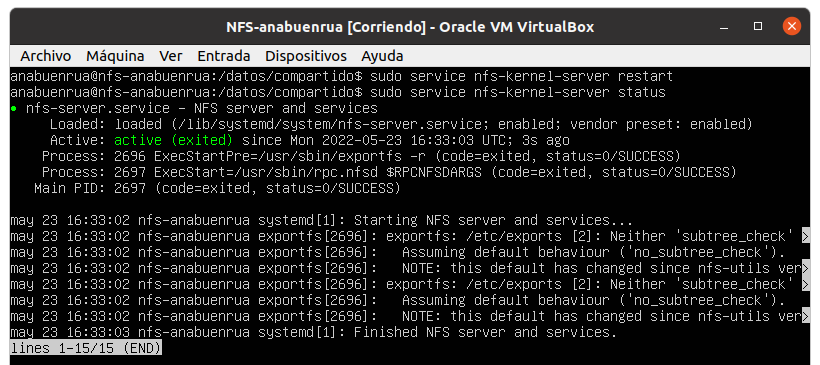
\includegraphics[scale=0.5]{config_5}
\end{center}
\end{figure}

Ahora vamos a configurar m1 y m2. Para no ser repetitivo, se va a realizar y mostrar la configuración solamente en m1, ya que en m2 se haría la misma.

Comenzamos instalando las herramientas que vamos a usar, como se ve en \eqref{config_6}

\begin{figure}[h!]
\begin{center}
\caption{Instalación de herramientas en m1}
\label{config_6}
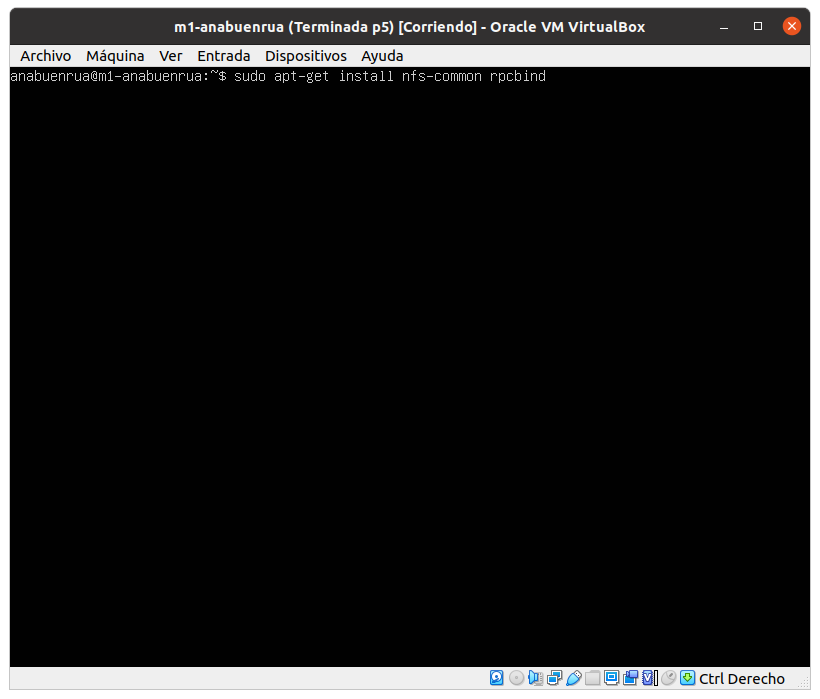
\includegraphics[scale=0.5]{config_6}
\end{center}
\end{figure}

A continuación creamos el punto de montaje datos en \verb|/home/anabuenrua|, le asignamos los permisos y montamos la carpeta remota, como se muestra en \eqref{config_7}.

\begin{figure}[h!]
\begin{center}
\caption{Creación del punto de montaje, asignación de permisos y montaje del directorio remoto.}
\label{config_7}
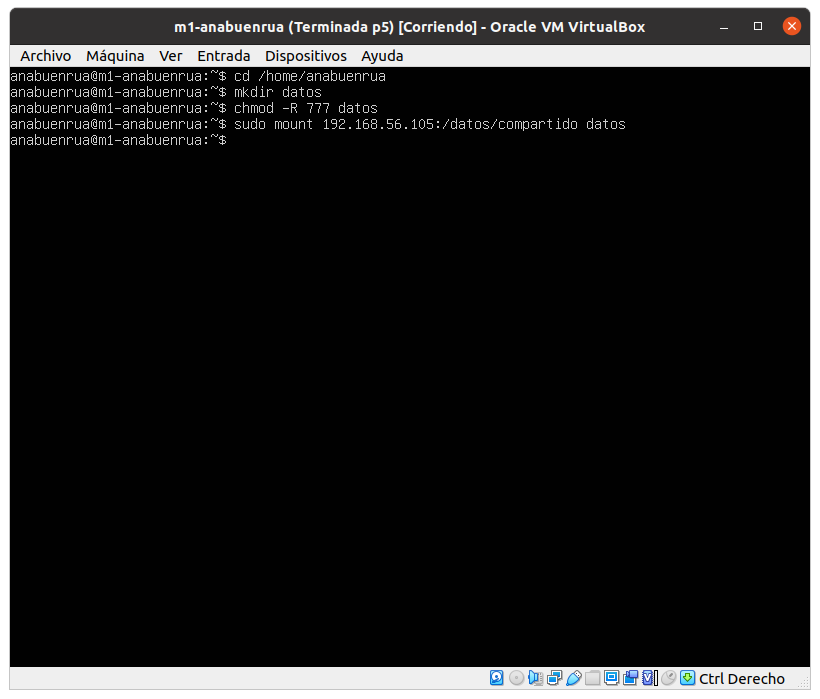
\includegraphics[scale=0.5]{config_7}
\end{center}
\end{figure}

Finalmente comprobamos que funciona, pues al crear un archivo en la carpeta datos de m1 se muestra en m2 y nfs. Esto puede verse en \eqref{config_8}.

\begin{figure}[h!]
\begin{center}
\caption{Comprobación del correcto funcionamiento.}
\label{config_8}
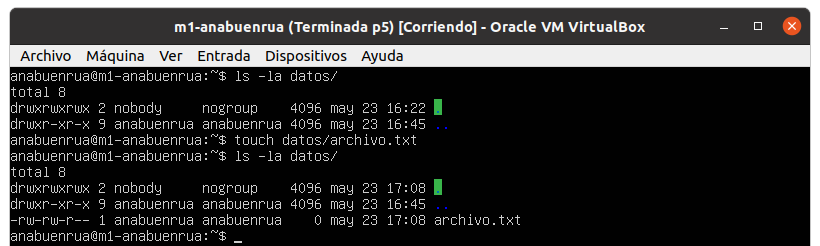
\includegraphics[scale=0.5]{config_10}
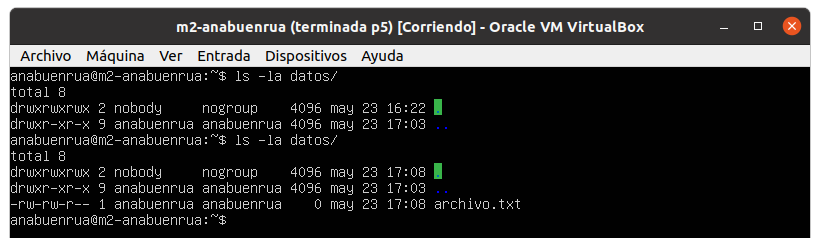
\includegraphics[scale=0.5]{config_11}
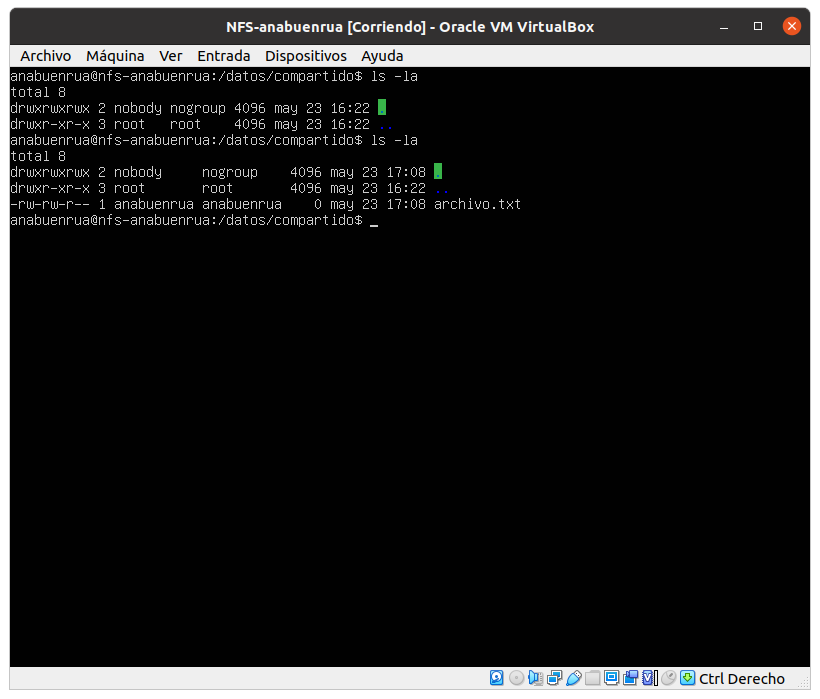
\includegraphics[scale=0.5]{config_12}
\end{center}
\end{figure}

\section{Opciones avanzadas}

Para comenzar, vamos a hacer que el montaje de la carpeta remota se realice de forma automática al arrancar la máquina virtual tanto en m1 como m2. Para ello, vamos a editar el fichero \verb|/etc/fstab| añadiendo la línea siguiente:

\begin{verbatim}
192.168.56.105:/datos/compartido /home/anabuenrua/datos/ nfsauto,noatime,
nolock,bg,nfsvers=3,intr,tcp,actimeo=1800 0 0
\end{verbatim}

Pese a que hemos tenido que mostrarla en 2 líneas, esta es una sola línea. El archivo editado puede verse en \eqref{config_9}.

\begin{figure}[h!]
\begin{center}
\caption{Fichero /etc/fstab}
\label{config_9}
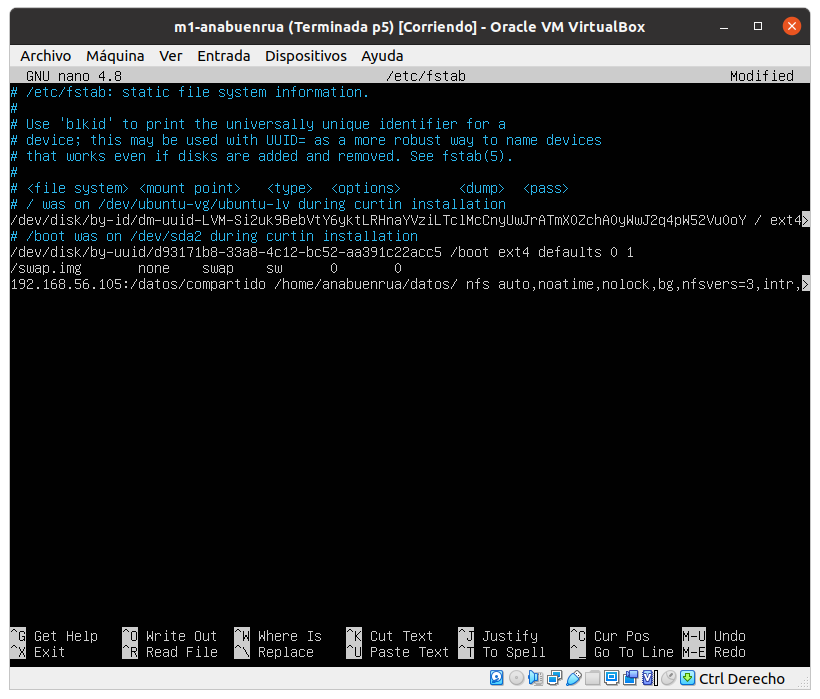
\includegraphics[scale=0.5]{config_8}
\end{center}
\end{figure}

Además, en la máquina nfs-anabuenrua podemos comprobar qué puertos se están usando como se ve en \eqref{config_10}.

\begin{figure}[h!]
\begin{center}
\caption{Puertos asignados.}
\label{config_10}
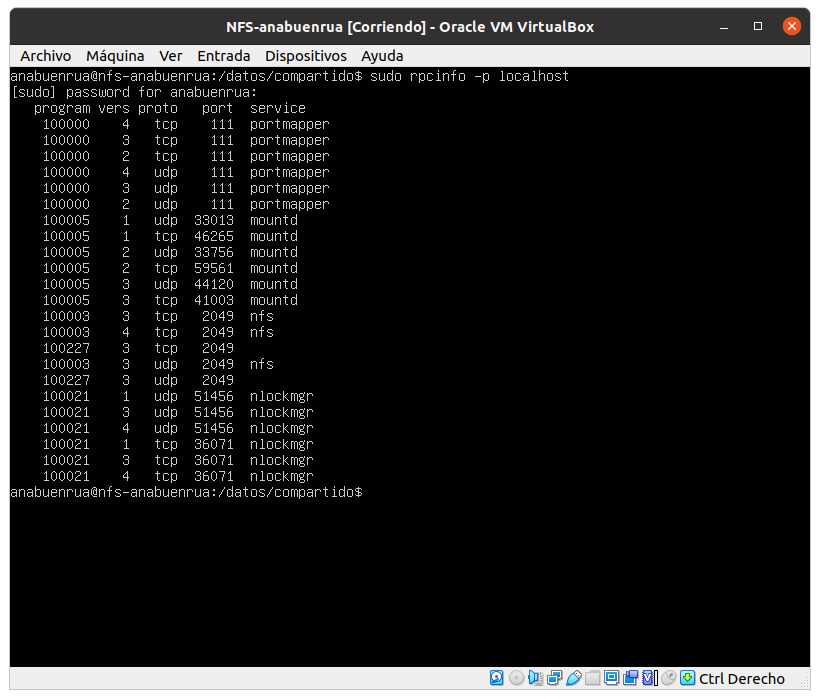
\includegraphics[scale=0.5]{config_9}
\end{center}
\end{figure}

\chapter{Seguridad en NFS}

Comenzamos creando en nfs-anabuenrua en \verb|/home/anabuenrua| una carpeta \verb|scripts_iptable| para almacenar los ficheros de configuración de iptables como en las otras máquinas.

Vamos a crear un fichero en esta carpeta que contenga las reglas de seguridad por defecto de esta máquina. Este fichero puede consultarse en \eqref{iptables_1}.

\begin{figure}[h!]
\begin{center}
\caption{Fichero de configuración básica de iptables.}
\label{iptables_1}
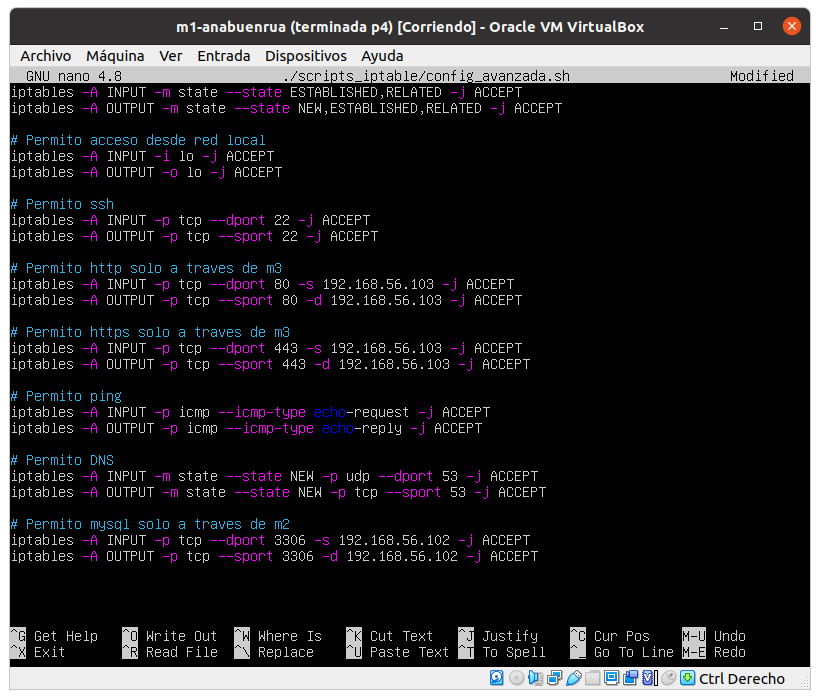
\includegraphics[scale=0.5]{iptables_1}
\end{center}
\end{figure}

\section{Opciones avanzadas}

Como mountd y nlockmgr usan puertos dinámicos para poder escribir reglas de iptables primero vamos a fijar los puertos de estos servicios.

Comenzamos fijando el puerto de mountd, para lo que editamos el fichero 

\verb|/etc/default/nfs-kernel-server| editando la línea correspondiente para fijar el puerto 2000 (por ejemplo, podríamos asignar otro). Este fichero puede verse en \eqref{iptables_2}.

\begin{figure}[h!]
\begin{center}
\caption{Fichero /etc/default/nfs-kernel-server.}
\label{iptables_2}
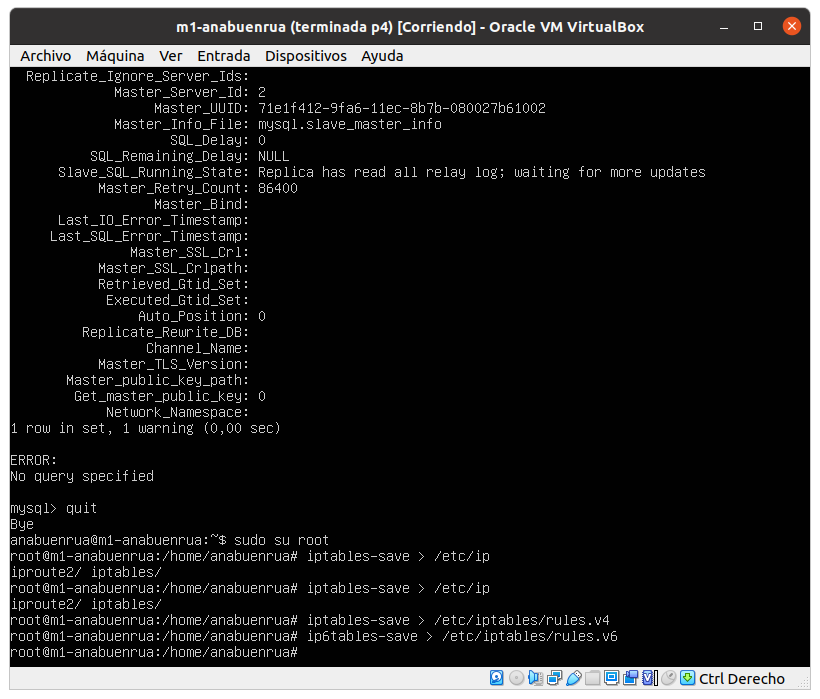
\includegraphics[scale=0.5]{iptables_2}
\end{center}
\end{figure}

Para fijar el puerto de nlockmgr creamos el archivo \verb|swap-nfs-ports.conf| en \verb|/etc/sysctl.d/| con el contenido que se muestra en \eqref{iptables_3} para fijar los puertos de tcp y udp a 2001 y 2002 respectivamente.

\begin{figure}[h!]
\begin{center}
\caption{Fichero /etc/sysctl.d/swap-nfs-ports.conf.}
\label{iptables_3}
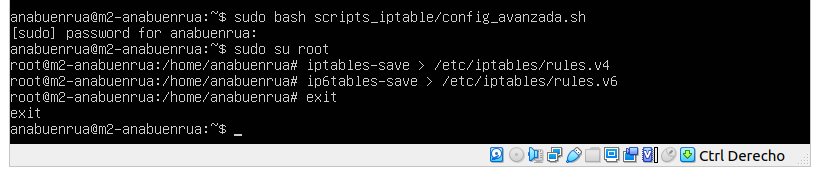
\includegraphics[scale=0.5]{iptables_3}
\end{center}
\end{figure}

Ahora reiniciamos el sistema especificando este archivo de configuración. En \eqref{iptables_4} se muestran los comandos empleados. Se omite la salida del primer comando debido a que es muy larga.

\begin{figure}[h!]
\begin{center}
\caption{Reinicio del sistema especificando el archivo de configuración.}
\label{iptables_4}
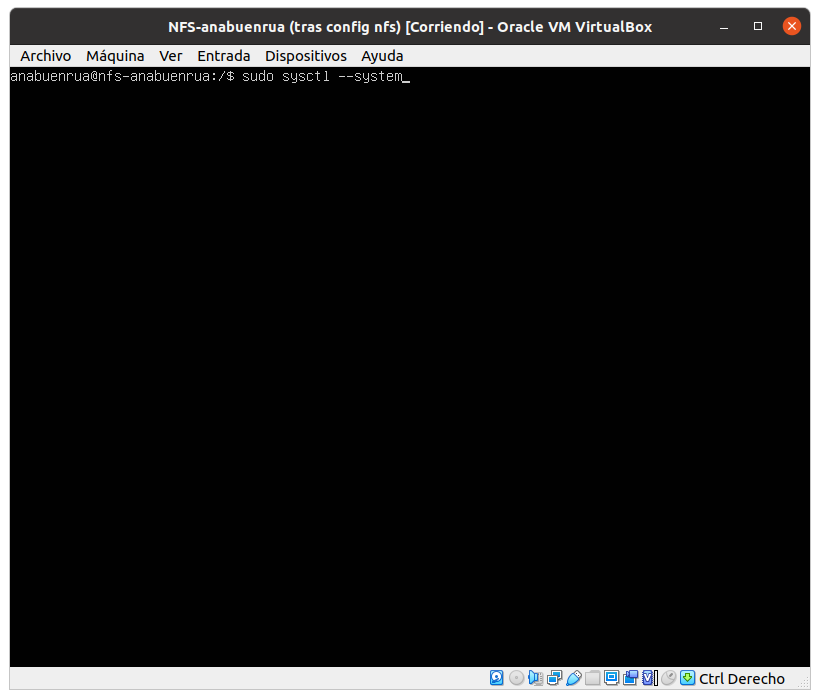
\includegraphics[scale=0.5]{iptables_4}
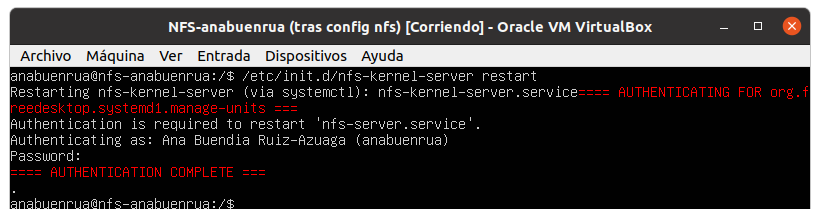
\includegraphics[scale=0.5]{iptables_6}
\end{center}
\end{figure}

Y comprobamos finalmente los puertos una vez realizada esta configuración. Esto puede verse en \eqref{iptables_7}

\begin{figure}[h!]
\begin{center}
\caption{Comprobación de puertos asignados.}
\label{iptables_7}
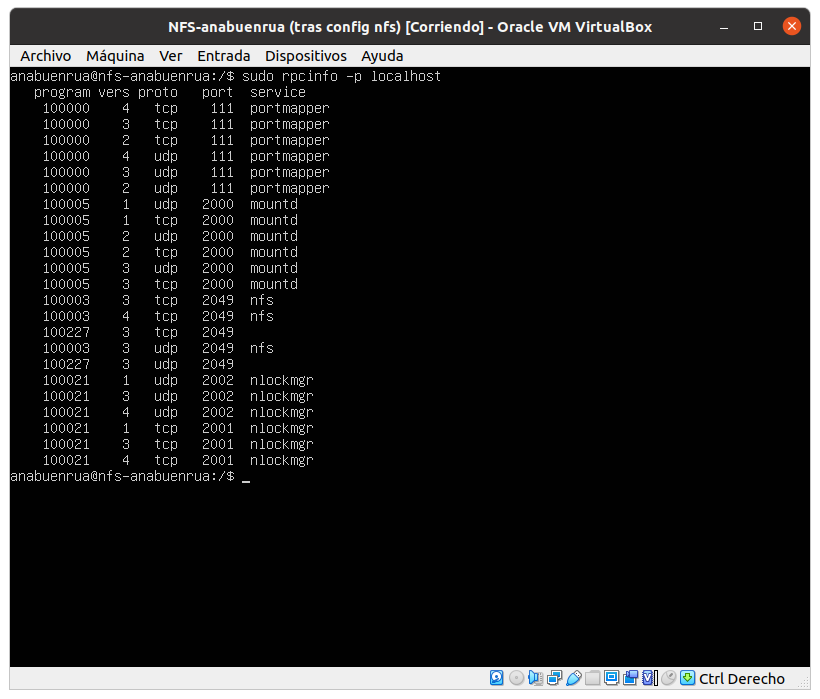
\includegraphics[scale=0.5]{iptables_7}
\end{center}
\end{figure}

Ahora que hemos fijado los puertos de estos servicios, podemos definir reglas para abrir los puertos correspondientes a estos. Partiendo del fichero de configuración ya presentado, lo editamos como se ve en \eqref{iptables_8}.

\begin{figure}[h!]
\begin{center}
\caption{Fichero de configuración avanzada de iptables}
\label{iptables_8}
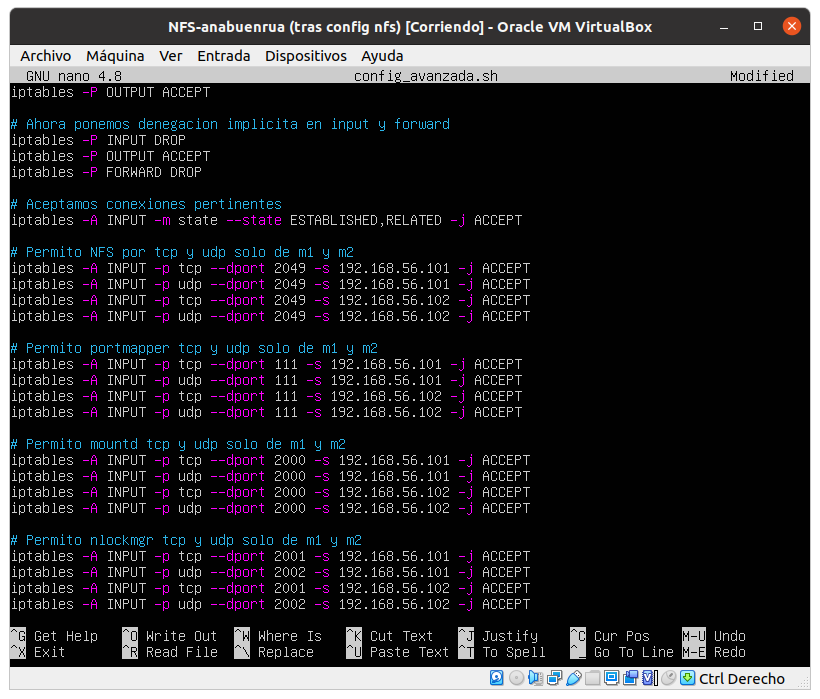
\includegraphics[scale=0.5]{iptables_8}
\end{center}
\end{figure}

Finalmente comprobamos que todo funciona correctamente repitiendo la prueba que puede verse en \eqref{config_8}.

Tras comprobar que la granja funciona correctamente y está bien protegida, usamos \verb|iptables-persistent| como hicimos en la práctica 4 (y se usó de nuevo en la 5) para hacer las reglas persistentes al inicio.



